
\cleardoublepage

\chapter{Results and Analysis}
\label{chapter:results}

The image-collection step of the experiment was successful, as was the effectiveness of the post-processing pipeline.  This chapter first discusses the final field map and then analyzes the different components of the post-process pipeline.  This includes QR code detection as well as the recursive splitting algorithm for finding plants.  The chapter concludes by looking at the accuracy of the mapped plants and codes, and a timing analysis of the entire mapping process.

\section{Field Map}

The final field map produced from the Kernza experiment is displayed in figure \ref{figure:field_map}.  This map is in the field coordinate system and shows the field is split into two different sections.  The split in the field was intentionally left un-planted to allow vehicles to drive from one end to the other.   The rectangle containing 15 rows labeled as 'special plants' refers to the plants that each have their own unique ID, as discussed in section \ref{section:field_setup}.  These were planted first, followed by the right portion of the field, and finally left section.  This explains why the two rows on the far left are 50 meters shorter than the rest. In addition, the right part of the field was shifted upwards 10 meters to avoid low quality soil.

\begin{figure}
	\centering
    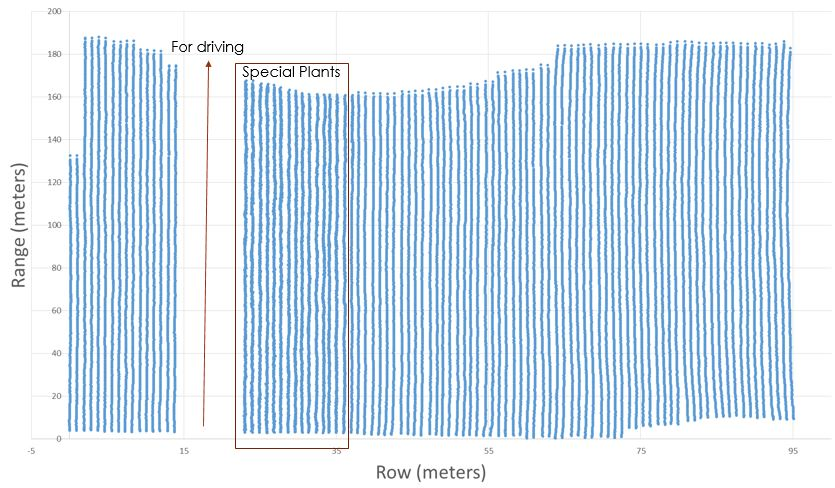
\includegraphics[width=6in]{figures/field_map.jpg}
    \caption[Field map]{Field map of Kernza showing both plants and QR codes as small blue circles.}
    \label{figure:field_map}
\end{figure}

\section{Code Detection}

The QR code detection proved to be robust. From the 4581 codes in the field, all but 2 were automatically detected by the first stage of the post-processing pipeline.  It is unknown why the 2 undetected codes were missed, but the most likely reasons are they were accidentally buried or did not appear in any images.  

However, 43 codes were not able to be read by the ZBar program.  Since each of the unreadable codes were placed in a special review directory, as described in section \ref{section:reading_codes}, it was straightforward to determine the reason each code couldn't be read.  The most likely cause was a printer error which resulted in a small section of the code to not be printed.  This printer error affected 25 of the 43 unreadable codes.  9 codes were partially blocked by field debris or insects sitting on the code.  7 had dirt on the code, which most likely splashed up during transplanting. And finally, 2 codes had too much glare to be read successfully.  Examples of each of these issues can be seen in figure \ref{figure:missed_codes}. 

\begin{figure}
	\centering
    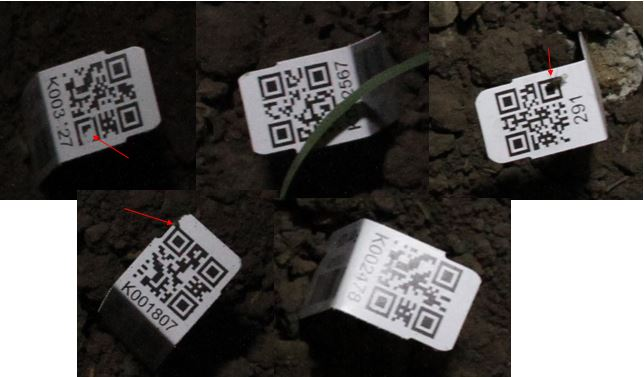
\includegraphics[width=5in]{figures/missed_codes.jpg}
    \caption[Unreadable QR codes]{Unreadable codes.  From left to right on top row: printer error, blocked by debris, blocked by fly. On bottom row: dirt, glare.}
    \label{figure:missed_codes}
\end{figure}

These unreadable codes were exported with their pixel coordinates and image name, which made it trivial to include them in the final results. The codes affected by printer error could be reduced by better inspecting the codes before planting or by using a different type of printer.  The glare issue could be eliminated by using a polarizing lens filter, however this would have the potential to change the white balance setting and also possibly reduce image sharpness.  Since the glare only affected 2 codes it is likely not worth the cost to address.  

\section{Plant Localization}
\label{section:plant_localization}

The number of plants in each group were manually counted before transplanting. However, it is unknown exactly how many plants ended up in the field because some plants were discarded during the transplanting process.  So the sum of the pre-counted plants, 25560, is the maximum number of plants that could be found in the field.  

The plant localization algorithm detected 24269 plants in the images and created 335 plants where no plant was detected, but where one should have been.  This resulted in a total of 24604 plants in the final map, which indicates 956, or roughly 1 out of every 25, plants were discarded during transplanting.  These results were considered reasonable for this experiment. 

Blue sticks were only found in 23\% of the plants that were detected in the images, however all plants should have had a blue stick marker.  The reason for this poor result was due to the lack of saturation in the blue sticks which made it difficult to find a threshold that didn't also detect the blue hues in the soil.  Also, there were variations in the intensity of the blue dye color that made it difficult to find a single set of threshold values for detecting the sticks.   

The assigned coordinates of the created plants were projected back onto images that contained those world coordinates, and an arbitrary 10 centimeter box was drawn on the image to indicate where the plant should have been.  Fifty of these images were manually analyzed and 46 of them closely matched an actual plant in the image that was either dead or mostly buried under soil.  The remaining 4 plants were either completely buried or a gap occurred in the field where nothing was planted.  

\section{Mapping Accuracy}

As discussed in section \ref{processing-stage5}, the coordinates of all the plants and QR codes had to be offset into the coordinate frame used by the Land Institute.  This was accomplished by manually surveying 10 codes using the Land Institute \ac{rtk} receiver and base-station, and then calculating the northing and easting offsets that would make the average error zero.  

After this offset is applied, the errors of the 10 surveyed codes were calculated and plotted in figure \ref{figure:code_errors}.  The reason that codes were used to calculate the offset, rather than plants, is it's easier for the post-processing to consistently identify the center of the code.  The average error is zero because that is how the shift in coordinates was calculated.  A good check would have been to use the robot's \ac{rtk} receiver to also survey the codes, but that was not realized until afterwards.

  \begin{figure}
	\centering
    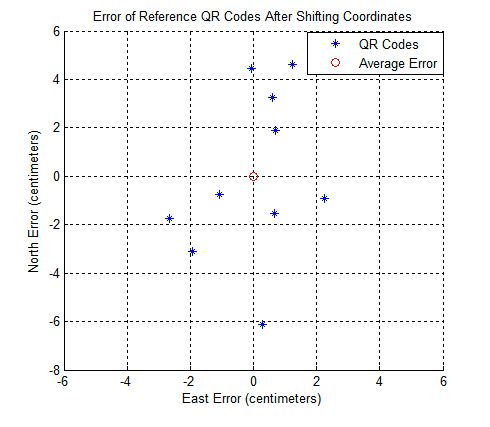
\includegraphics[height=4in]{figures/code_errors.jpg}
    \newline
    \newline
    \centering
    \begin{tabular}[c]{|c|c|c|}
       \hline
        Error & East (cm) & North (cm) \\ 
        \hline
        Average   & 0 & 0             \\
        $|$Average$|$ & 1.4 & 3.4       \\
        Std. Dev. & 1.5 & 3.5         \\
        $|$Maximum$|$   & 2.8 & 7.2       \\
        $|$Minimum$|$   & 0.5 & 0.8       \\
        \hline
    \end{tabular}
    \captionlistentry[table]{Position errors of QR codes}
    \captionsetup{labelformat=andtable}
    \caption[Errors in reference QR codes]{Errors in reference QR codes after shifting to the Land Institute coordinate system.}
    \label{figure:code_errors}
  \end{figure}

An additional 20 plants were surveyed to verify that their mapped positions were accurate enough to distinguish them from their neighboring plants.  As with the surveyed codes, the plants were chosen randomly and evenly distributed throughout the field.   A similar plot showing the errors for each surveyed plant can be seen in figure \ref{figure:plant_errors}.  The average error is relatively small, which shows the offsets calculated using the codes weren't biased.   

  \begin{figure}
	\centering
    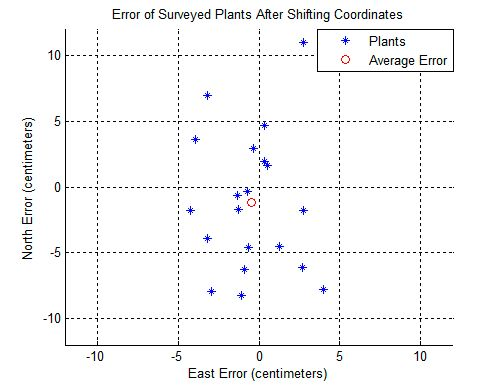
\includegraphics[height=4in]{figures/plant_errors.jpg}
    \newline
    \newline
    \centering
    \begin{tabular}[c]{|c|c|c|}
        \hline
        Error & East (cm) & North (cm) \\ 
        \hline
        Average   & -0.5 & -1.2           \\
        $|$Average$|$ & 2.1 & 4.5       \\
        Std. Dev. & 2.4 & 5.3       \\
        $|$Maximum$|$   & 4.3 & 10.9       \\
        $|$Minimum$|$   & 0.3 & 0.6       \\
        \hline
    \end{tabular}
    \captionlistentry[table]{Position errors of plants}
    \captionsetup{labelformat=andtable}
    \caption[Errors in surveyed plants]{Error between mapped and manually surveyed plants.}
    \label{figure:plant_errors}
  \end{figure}

The largest source of errors from these measurement are errors in assigning an accurate time-stamp to each image.  These timing errors are primarily caused by camera latency as well as latency in the \ac{gnss} receiver.  Camera latency is the amount of time between when the data collection program commands the camera to take an image, and when the image is actually exposed.  \ac{gnss} latency is the amount of time between when a position is calculated by the receiver, and when it is received by the data collection program. 

From experimental testing the camera latency was determined to have a latency following a normal distribution with a mean of 65 milliseconds and a standard deviation of 30 milliseconds.  The mean latency can be accounted for in the data collection program, but the variance can not. The \ac{gnss} receiver was configured to output at 50 hertz and a baud rate of 115200 bits per second.  This results in an estimated latency in the range of 20 to 30 milliseconds.  Combining these latencies with the platform motion results in an error of:
\begin{align*}
 \text{error} &= L (s + \dot{\psi}*d) \\
             &= .06 \text{ sec}* (40\text{ cm/sec} + 0.2 \text{ rad/sec} * 80 \text{ cm}) \\ 
             &= 3.4 \text{ cm}
\end{align*}
where $L$ is the combined latency, $s$ is the nominal platform speed, $\dot{\psi}$ is the average yaw rate needed to keep the platform between the rows, and $d$ is the distance from the platform center of rotation to the camera.  This assumes the camera's have a level orientation, which is the case for the robot.  While this is a rough estimate, it shows that the error is a significant contribution to the overall error.

The contributions of error from vehicle speed is twice as large as that from the platform rotation. Forward motion of the robot was primarily in the northing direction which explains why these errors are around twice as large as the easting direction.  Another contributing factor is the estimation error in the \ac{gnss} position and heading.

The additional errors in the surveyed plants compared to the codes is likely due to a larger discrepancy between what the post-processing pipeline detects as the center of a plant and what a human measures as the center of the plant. 

\section{Plant Spacing}

An additional check to verify the results is that the plant spacing should be consistent with the output rate of the transplanter.  The histogram below shows the distribution of plant spacing for all the plants.  As expected the mean plant spacing is 25.7 inches, which is close to the expected 24 inches. However, the variances in plant spacing highlights the importance of mapping individual plants, and not assuming the transplanter outputs at a consistent rate.

\begin{figure}
	\centering
    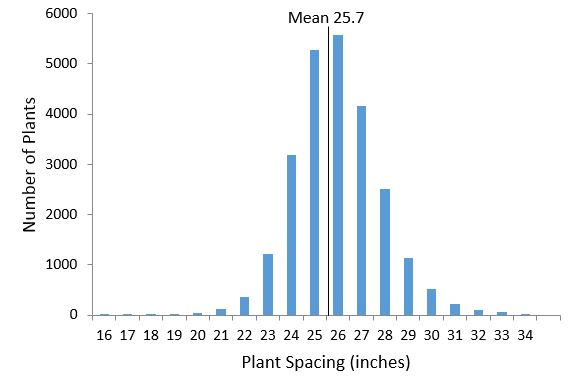
\includegraphics[width=5in]{figures/plant_spacing.jpg}
    \caption[Plant spacing histogram]{Histogram of spacing between successive plants.}
    \label{figure:plant_spacing}
\end{figure}

\section{Time Analysis}

An important consideration to the success of the mapping system is how much time it takes to collect and analyze all of the images. For this experiment, the robot speed and camera triggering rate were set as described in section \ref{section:determining_parameters}.  This resulted in a total driving time of approximately 10 hours spread over 4 different nights.  Each night required 30 minutes for setup and another 30 for tear-down, which added in a total of 4 additional hours.  

During the 10 hours of driving, the robot collected 54,512 images.  The timing analysis for the post-processing are presented in table \ref{table:timing_analysis}. These results were bench-marked on a Lenovo S431 ultra-book running a dual core i7-3687 at 2.6 gigahertz with 8 gigabytes of random access memory.  

\begin{table}
    \begin{center}
    \begin{tabular}[c]{|c|c|c|}
        \hline
        Stage & Time Per Image (sec) & Total Time (hours) \\
        \hline
        Extracting QR Codes & 0.9 & 13.6   \\
        Creating Field Structure & - & 0.05   \\
		Extracting Plant Parts & 1.0 & 15.1   \\
		Locating Plants & 0.005 & 3   \\
		Saving Field Map & - & 0.05   \\
		\hline
		\textbf{Total} & \textbf{1.9} & \textbf{31.7}   \\ 
        \hline
    \end{tabular}
    \caption[Post-processing time analysis]{Timing analysis for each stage of the post-processing pipeline.}
    \label{table:timing_analysis}
   \end{center}
\end{table}

One thing to note is it's straightforward to run the first stage in parallel for each night that images were collected.  Also, if extracting plant parts were combined with the first stage, this would result in a large reduction in overall processing time.  
